\chapter{System Design}
\label{chp:chap-four}

\section{WiFi Controller Design}

\section{Smart Contract Design}

The two major components are the WiFi controller and the smart contract. The smart contract  calculates the bandwidth allocation and collects payments. The WiFi controller allocates the correct bandwidth to each user. Before introducing each part in detail, an analysis is given between system design of traditional app and DApp.

\section{Tradition App and DApp}
Roughly, our proposed system can be considered as a web application with blockchain smart contract, which follows the definition of the DApp\cite{johnston_general_nodate}. DApp, stands for Decentralized Application, which would be introduced in detail in Chapter. \ref{chp:chap-five}. And a typical web application is a group of code such as html, javascript and css. As this group of code running on users' personal devices, a browser, users can interact with the application to fulfill their demands.

And normally when you interact with a web application, you use a web browser to connect to a central server over a network. All the code of this web application lives on this central server, and all the data lives in a central database. Anytime you transact with your application, must communicate with this central server on the web. This is what happened while using the traditional web applications. And the system structure of this kind of web application is shown in  Fig.\ref{fig:app}

\begin{figure}[h]
    \centering
    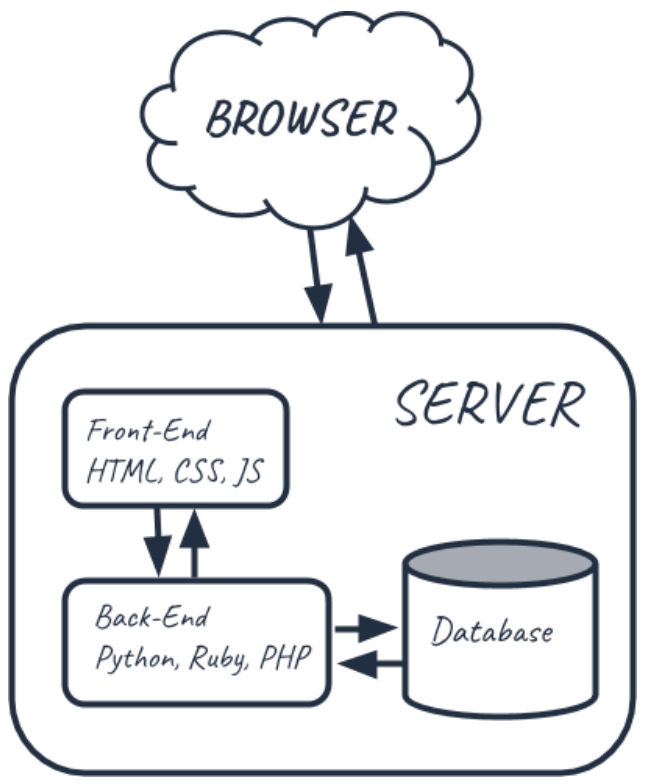
\includegraphics[width=5cm]{My-Thesis/figures/traditional_web_application.png}    
    \caption{Traditional App System Structure}
    \label{fig:app}
\end{figure}
\begin{figure}[h]
    \centering
    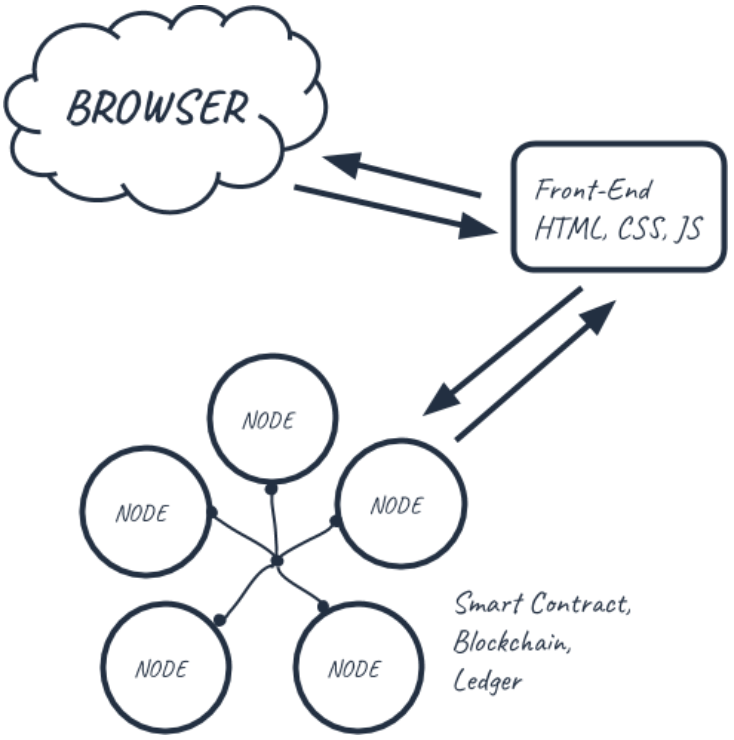
\includegraphics[width=5cm]{My-Thesis/figures/dapp_structure.png}    
    \caption{DApp System Structure}
    \label{fig:dapp}
\end{figure}

And this traditional and widely used kind of web application is very intuitive to develop and holds a great performance while having a powerful central server. However even as concurrent server frameworks are already well developed in decade, a single centralized server always have a limit number of users it can interact with at the same time. And when the central server shut down, the whole system shut down. While, the system structure of a DApp system holds a great elasticity and a robustness while facing the rapidly growing number of user. However, this defect of traditional structure can be solved with a "centralized" distributed servers, which runs the traditional system structure on a distributed group of server instance.

But more importantly, the main reason that the concept DApp was published by scholars is that it can achieve some application scenarios that a traditional app can not support. And in such scenarios, the properties that a traditional web application holds may become the drawbacks. Taking our use case, bidding system, as an example, while implementing the bidding system on a centralized server like Fig.\ref{fig:app}, it will run into two problems as following:
\begin{addmargin}[2em]{0em}

The data on the database could be changed: it could be counted more than once, or removed entirely. \newline The source code on the web server could also be changed at any time.
\end{addmargin}
